
\thispagestyle{empty}

\begin{center}
\Large
%Introduction
Préambule
\normalsize
\end{center}
\vspace{1cm}

Ce document souhaite donner un aperçu élémentaire de la
philosophie à propos de la croyance, du doute et de l'opinion.


Le premier chapitre est extrait du {\it nouveau vocabulaire de la philosophie} d'Armand Cuvillier.

Les chapitres suivants sont extraits de {\it La pratique de la philosophie} (destiné aux
lycéens), et de l'{\it encyclopédie de la philosophie} de Garzanti (destinée aux néophytes).

%\vspace{1.3cm}
\vfill

\begin{center}
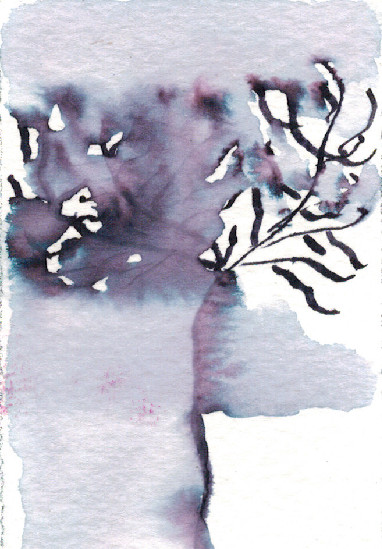
\includegraphics[scale=0.5]{./presentation/gauche2}
\hspace{1cm}
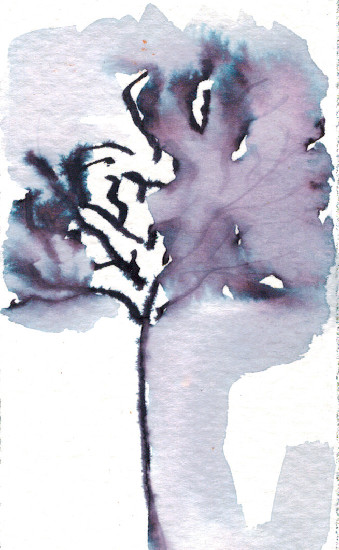
\includegraphics[scale=0.5]{./presentation/droite2}
\end{center}

%« Chaque fois que les gens s’interrogent "Mais qu’est-ce donc que la vérité ?" – en général, c’est parce que la vérité est juste sous leur nez, mais il serait fort incommode d’en convenir. Et aussi, à l’encontre de sa conviction intime, Pilate cède à la volonté de la foule et lui abandonne Jésus pour qu’il le crucifie. Le problème pour Pilate n’était pas déterminer si Jésus était innocent. Cette question-là était facile à trancher. Non, le vrai problème est que, en fin de compte – comme nous tous, la plupart du temps –, la vérité était devant lui, mais il a préféré s’en laver les mains. »

%Simon Leys, Le bonheur des petits poissons. Lettres des Antipodes, éd. JC. Lattès, 2008
%\vspace{2.3cm}
\vfill
\vspace{1.7cm}

\hfill {\it Les documents de Zécriture}

\hfill \texttt{www.zecriture.fr}

\vspace{0.7cm}


\hfill Numérisation : Stephan Runigo

\hfill Illustrations : Christiane Audhuy

%%%%%%%%%%%%%%%%%%%%%%%%%%%%%%%%%%%%%%%%%%%%%%%%
